\section{Modèle théorique de Mumford Shah}

Ce modèle est l'un des plus étudié. La fonctionnelle de Mumford-Shah a été introduite en 1989. D'un point de vue continue, une image est vue comme une fonction $g : \Omega \rightarrow \mathbb{R}$, où $^Omega$ est par exemple un rectangle, et $g$ associe à chaque point $x \in \Omega$ de l'image une valeur $g(x)$ qui représente un niveau de gris. La fonction g n'est pas régulière, elle est très souvent discontinue. c'est cet effet de discontinuité qui nous intéresse. En effet, nous voulons trouver pour une image $g : \Omega \rightarrow \mathbb{R}$ l'ensemble des contours des objets que représente l'image. Ces contours sont dont localisés au points de discontinuités de g : il y a une franche discontinuité dans les niveaux de gris.

Pour résoudre ce problème, Mumford et Shah introduisent une fonctionnelle qui par minimisation, va chercher les points de $g$ les plus discontinus.

\bigskip

Le problème s'écrit alors : 
\[\underset{(u, K) \in \mathcal{A}(\Omega)}{min} \; \; \; J(u,K) := \int_{\Omega \backslash K} |u - g |^2 dx + \int_{\Omega \backslash K} ||\nabla u ||^2 dx + \mathcal{H}^1(K) ,  \]

avec 
\[ \mathcal{A} (\Omega) = \{ (u,K) : K \subset \Omega \; \; \; \text{est fermé et } \; \; \; u \in C^1(\Omega \backslash K) \} \] 

Nous pouvons expliciter chacun des termes qui composent cette fonctionnelle :
\begin{itemize}
\item $\int_{\Omega \backslash K} |u - g |^2 dx $ force u, par minimisation, à ressembler le plus possible à l'image de départ g.

\item $\int_{\Omega \backslash K} ||\nabla u ||^2 dx $ pénalise les oscillations de u, qui par minimisation, forcera u a être la plus régulière possible. Comme g est très irrégulière au début, on ne peut pas avoir $ u = g$ partout dans $\Omega$. 
Ainsi, l'ensemble K possède un rôle essentiel : s'il est bien positionné sur les singularités de $g$, il permettra de minimiser le premier terme décrit ci-dessus.

\item $\mathcal{H}^1(K) $ désigne la mesure de Hausdorff de dimension 1 de l'ensemble $K$. Ce dernier terme force $K$ à être de dimension de Hausdorff $1$, qui nous donne bien l'intuition d'un "contour". Par exemple, un cercle est de dimension de Hausdorff 1. 
Cet ensemble $K$ devra être optimisé pour couvrir le plus possible les singularités de $g$, en le positionnant en priorité sur les discontinuités les plus franches. 
Les autres singularités non prise en compte dans ce terme, donc minimes, seront considérés en oscillations. $\mathcal{H}^1(K)$ est la mesure de Lebesgue sur $\mathbb{R}$.
\end{itemize}


\subsection{Mesure et dimension de Hausdorff : compléments}
Les mesures de Hausdorff sont une généralisation des notions de longueur, d'aire, de volume... $\mathcal{H}^n$ est la mesure de Lebesgue en dimension $n$ pour des sous ensembles de $\mathbb{R}^n$, multipliée par une constante qui n'est autre que le volume $n-dimensionel$ de la boule unité.

\bigskip

La mesure de Hausdorff peut être définie pour tout ensemble. Pour un sous-ensemble non-vide $U$ d'un espace euclidien de dimension $n$, on peut définir le diamètre de $U$ tel que : 

\[ diam \; \; U  =  |U| = sup\{ |x-y| \;  :  \; x,y \in U \}\] 
Avec la distance euclidienne usuelle.

\bigskip

Ensuite, si un ensemble F est recouvert par une collection dénombrable $\{U_i\}$, de diamètre au plus $\delta$ : 

\[ F = \cup_{i=1}^{\infty} U_i \; \; \; \text{avec}\; \; \; 0 < |U_i| \leq \delta  \]
 On dit que $\{U_i\}$ est un $\delta$-recouvrement de $F$.
 
\bigskip
 
Soit maintenant un $s \in \mathbb{R} >0 $. Pour tout $\delta >0$, on peut définir : 

\[ \mathcal{H}_{\delta}^s (F) = inf \{ \sum \limits_{i=1}^{\infty} |U_i|^s \; : \; \{U_i\} \text{est un recouvrement de } F\}\].

Ainsi, 

\[ \mathcal{H}^s (F) = \underset{\delta -> 0}{lim} \mathcal{H}_{\delta}^s (F)\] 

Et $\mathcal{H}^s (F)$ est appelé la mesure de Hausdorff s-dimensionnelle de $F$.

\bigskip

$\textit{Théorème 1 : Dimension de Hausdorff (admis)}$ : Soit $F$ un sous-ensemble. Il existe un unique  $d \in \mathbb{R}_{+} \cup {\infty}$ tel que : 
\[ 1. \; \; \mathcal{H}^s (F) = \infty \; \; \; \text{pour tout} \; \;  s<d \] 
\[ 2. \; \; \mathcal{H}^s (F) = 0 \; \; \; \text{pour tout} \; \; s>d \] 

On appelle dimension de Hausdorff de $F$ le réel $d$. C'est la valeur critique de s pour laquelle la mesure passe de $0$ à $\infty$.

\bigskip

On l'appelle également dimension fractale. 

\begin{figure}[H]
\centering
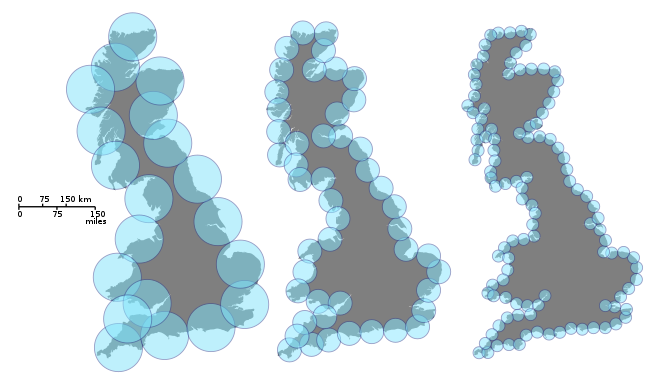
\includegraphics[scale=0.5]{images/hausdorff.png}
\caption{Dimension de Hausdorff de la Grande Bretagne }
\end{figure}


